\documentclass[a4paper, 10pt]{report}

\usepackage[utf8]{inputenc}
\usepackage{mathtools}
\usepackage{amsmath}
\usepackage{amsfonts}
\usepackage{graphicx}
\usepackage{tabularx}
\usepackage{listings}
\usepackage[table]{xcolor}
\usepackage{tikz} 

\usepackage[italian]{babel}

\usepackage{hyperref}
\usepackage{geometry}
\geometry{
a4paper,
total = {170mm, 240mm},
left = 20mm,
top = 20mm,
}

\definecolor{codegreen}{rgb}{0,0.6,0}
\definecolor{codegray}{rgb}{0.5,0.5,0.5}
\definecolor{codepurple}{rgb}{0.58,0,0.82}
\definecolor{backcolour}{rgb}{0.95,0.95,0.92}

 
\lstdefinestyle{pretty_sql}{
    backgroundcolor=\color{backcolour},   
    commentstyle=\color{codegreen},
    keywordstyle=\color{magenta},
    numberstyle=\tiny\color{codegray},
    stringstyle=\color{codepurple},
    basicstyle=\ttfamily\footnotesize,
    breakatwhitespace=false,         
    breaklines=true,                 
    captionpos=b,                    
    keepspaces=true,                 
    numbers=left,                    
    numbersep=5pt,                  
    showspaces=false,                
    showstringspaces=false,
    showtabs=false,                  
    tabsize=2,
    language=sql
}

\lstset{style=pretty_sql}

\newtheorem{assioma}{Assioma}

\newtheorem{exmp}{Example}[section]

\setlength{\parskip}{0.5em}
\setlength{\parindent}{0pt}

\title{Appunti di \textit{"Basi di Dati"}}
\author{Alessandro Massarenti}
\date{Gennaio 2022}

\begin{document}

\maketitle

\tableofcontents

\chapter{Il modello relazionale}

Il modello di base di dati relazionale è il modello più utilizzato per rappresentare ed organizzare una base dati. Questo modello si basa sul concetto matematico di relazione, ovvero la connessione tra dati è relazionata per mezzo dei valori.

Quindi, su dominio:
\[D_1, D_2, ..., D_n\]

Posso avere relazioni:

\[D_1  \times D_3\]
\[D_2  \times D_3\]
\[D_4 \times D_1\]

\section{Caratteristiche}
Questo tipo di relazione e quindi di modello ha varie caratteristiche interessanti e peculiari.

\begin{itemize}
    \item Non c'è ordine tra le righe
    \item non c'è ordine tra le colonne
    \item le righe sono tutte diverse tra loro
    \item le intestazioni sono diverse tra loro
    \item i valori contenuti nelle colonne sono dello stesso dominio.
\end{itemize}

Inoltre, come dicevamo prima la connessione tra le varie relazioni è fatta per mezzo dei valori. Sarà quindi possibile collegare i dati e creare un'informazione più estesa ed importante.


\begin{exmp}\

    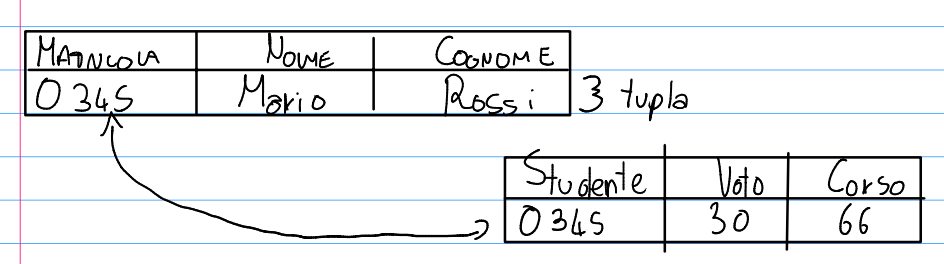
\includegraphics[width=\textwidth]{img/con_tra_rel.png}
\end{exmp}


\section{Tuple}

\begin{assioma}
Data la relazione $ R(A_1 , ..., A_n)$, una tupla è una funzione che definisce la relazione tra i vari dati. 
\end{assioma}

Le tuple vengono rappresentate come le righe delle tabelle in un database relazionale. Al singolare, una riga si chiama tupla.

Vedremo poi che una tupla è il risultato di una query, quindi non è solamente una riga della tabella se per ottenere più informazione uniamo i dati presenti in più tabelle.


%%Non chiaro
\begin{assioma}
Istanza di relazione su uno schermo $R(x)$ un insieme di tuple su $X$
\end{assioma}
%%------

\section{Valore NULL}

Il valore NULL è un valore che non fa parte del dominio, però è utile per definire dei campi in cui i dati non sono presenti.

\begin{description}
	\item[N.B.] Bisogna usare NULL con attenzione, perchè non facendo parte del dominio potrebbe dare comportamenti inattesi.
\end{description}

Per non tollerare valori nulli nel mio dominio dovrò utilizzare dei costraint.

\section{Risoluzione delle ridondanze}

Per risolvere le ridondanze, ovvero la duplicazione di dati nelle tabelle, si utilizzano i vincoli.

\section{Vincoli di integrità}

\subsection{Rigetto semantiche scorrette}
Nei database relazionali posso rigettare semantiche scorrette.

\includegraphics[width=\textwidth]{img/vincoli_di_integrità.png}

Alcuni tipi di vincoli sono supportati dal DBMS\footnote{Database management system}
Altri vincoli non sono supportati dal DBMS e vengono quindi mantenuti client side.

\subsection{Vincoli inter-relazionali}

I vincoli inter-relazionale è un vincolo che coinvolge più tabelle.

Se controllo l'integrità solo tramite vincoli di questo genere potrei però avere delle ridondanze, per questo si usa il vincolo di chiave.

\section{Vincoli di chiave}
Il vincolo di chiave dice che non posso avere tuple con i campi chiave uguali, ad esempio il codice fiscale che non può essere lo stesso per più persone.

Le chiavi verranno usate per gestire le relazioni tra tuple.

\subsection{Super-chiavi}

Un insieme $\mathbb{K}=\left\{K_1 , ..., K_n \right \} $ è una super chiave se non esistono tuple con gli stessi valori.

Una super-chiave identifica le tuple di una relazione.

Esiste infatti sempre almeno una super-chiave ed è \textbf{"tutta la tupla"}

\subsection{Chiavi}

Vedremo più in dettaglio le chiavi nel capitolo dedicato, capitolo \ref{chap:chiavi}

Una chiave è una super-chiave minimale quando:

\[\mathbb{K} \text{super-chiave è chiave} \leftrightarrow \forall k \mid k-k \text{ Non è superchiave} \]

Questa cosa va controllata che sia valida per ogni valore possibile e non solo per i valori attuali.

\begin{exmp}

Qui abbiamo un esempio delle chiavi.

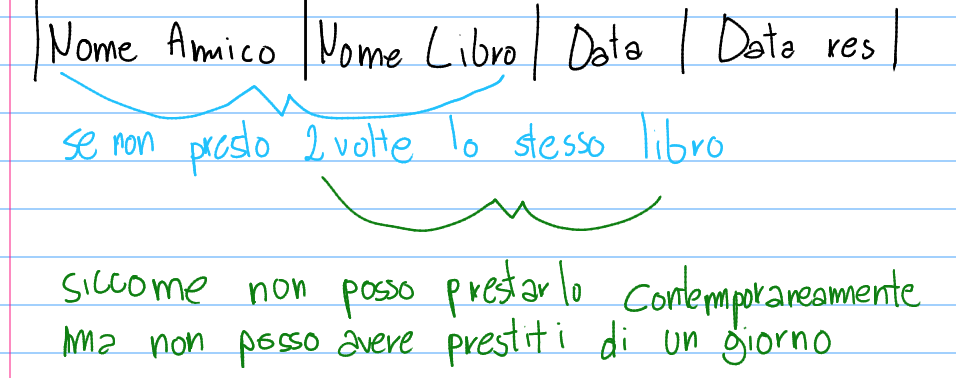
\includegraphics[width=\textwidth]{img/esempio_chiavi.png}

In questo caso infatti $(NomeAmico,NomeLibro)$ è chiave se non posso prestare allo stesso amico lo stesso libro più volte.

Nella seconda parte dell'esempio invece se $(NomeLibro,Data)$ è chiave non posso prestare lo stesso libro più volte nello stesso giorno.
\end{exmp}



\chapter{Chiavi} \label{chap:chiavi}

\section{Chiavi primarie}
La chiave primaria è la chiave principale della tabella, serve per identificare l'unicità di una riga in una tabella.

Se la chiave è formata da più campi deve essere riportata tutta quando è utilizzata come chiave esterna.

La chiave primaria non ammette valori nulli.

\section{Chiavi esterne}
Una chiave esterna deve comparire come chiave primaria nella tabella referenziata.

Una chiave esterna può essere anche \textit{NULL}

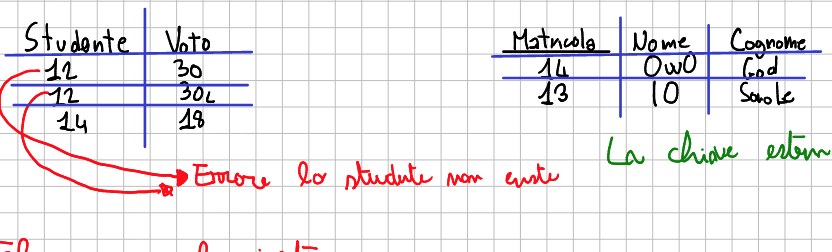
\includegraphics[width=\textwidth]{img/chiave_esterna.png}

\subsection{Eliminazione di chiavi esterne}

L'eliminazione di chiavi esterne è una situazione molto pericolosa e piena di insidie, va quindi eseguita con cura per mantenere l'integrità del dominio che si sta rappresentando nella base dati.

Le modalità di eliminazione di dati inseriti nel contesto delle chiavi esterne sono di vari tipi:

\begin{itemize}
    \item On delete cascade, ovvero elimino tutti i dati che utilizzano la chiave esterna.
    \item Assegnazione di \textit{NULL}
    \item Errore di eliminazione, ovvero devo prima eliminare manualmente i dati che utilizzano la chiave esterna.
\end{itemize}

\section{Super-chiavi}

Le super-chiavi permettono di capire di quale riga stiamo parlando. Sarà importante che una riga sia sempre super-chiave, questo determina infatti la non ridondanza dei dati nella tabella.

\begin{description}
	\item[N.B.] Più la super-chiave è piccola, e interessa quindi meno campi, meglio è, infatti più la super-chiave è piccola più è ampio l'insieme di dati che possiamo salvare.
\end{description}
\chapter{Algebra relazionale}

L'algebra relazionale è un linguaggio atto a definire in maniera chiara e matematica le relazioni tra i dati.

Abbiamo quindi la differenza tra:

\begin{itemize}
    \item DDL: data definition language
    \item DML: data manipulation language
\end{itemize}

Le relazioni saranno definite come il semplice prodotto cartesiano tra insiemi.

\section{Operatore Unione}
L'operatore di unione è l'unione matematica di due insiemi, si avrà quindi come risultato tutti gli elementi degli insiemi uniti togliendo i duplicati.

Questo operatore è rappresentato dal simbolo $\cup$.

\section{Operatore intersezione}
L'operatore di intersezione sono, come in matematica, gli elementi comuni agli insiemi intersecati.

Questo operatore è rappresentato dal simbolo $\cap$.
\section{Differenza}
Considerando due insiemi, $A$ e $B$, l'operazione di differenza ritorna solo gli elementi presenti in $A$ e non in $B$.

Questo operatore è rappresentato dal simbolo $\subset$.

\section{ridefinizione}

Ho una ridefinizione quando cambio un'intestazione della tabella.

In inglese questa operazione viene definita come \textit{"Rename"}.

Questo operatore è rappresentato dal simbolo $\rho $\footnote{Rho}.

\section{selezione}

Quando prendo un sottoinsieme delle tuple faccio una selezione.

Rappresento questo operatore con $\sigma $\footnote{Sigma}

\begin{exmp}

Ecco qualche selezione d'esempio:

$\sigma \text{stipendio} > 50$;

$\sigma \text{stipendio} > 50 \wedge \text{nome}=\text{"Mario"}$;
\end{exmp}

\section{proiezione}

Sto facendo una proiezione quando prendo un sottoinsieme della tupla. Le proiezioni eliminano i duplicati.


\begin{description}
	\item[N.B.] Siccome eliminano i duplicati è bene farlo sulle super-chiavi.
\end{description}

Le proiezioni si rappresentano con il simbolo matematico $\Pi$\footnote{Pi} ovvero project.

%Da espandere di molto la sezione
\section{join}

Quando faccio una join prendo 2 relazioni e unisco le tuple su attributi uguali.

Un join è completo se faccio proiezioni sugli operandi riottengo i primi, non è completo se alcuni campi non corrispondono.

Il join ri rappresentano con il simbolo $\bowtie$.

Esistono poi più tipologie di join:
\begin{itemize}
    \item join esterno
    \item semi join
    \item join cartesiano, detto anche join naturale
    \item theta join
\end{itemize}



\subsection{Join esterno}

In un join esterno mantengo gli $R_1$ senza match mettendo i corrispondenti a \textit{NULL}

\begin{exmp}
\[ R_1 \bowtie _{LEFT} R_2  \]
\end{exmp}

\subsection{Semi join}

\begin{exmp}
\[ R_1 \bowtie _{SEMI} R_2 = \Pi _R1\left( R_1 \bowtie R_2 \right)   \]
\end{exmp}

\subsection{Join cartesiano, detto anche join naturale}

Join senza match tra attributi

\subsection{Theta join}
\[ R_1 \bowtie _{COND} R_2 = \sigma cond \left(R_1 \bowtie R_2 \right) \]

\chapter{Viste}\label{chap:viste}

Le viste sono una rappresentazione differente degli stessi dati, servono per rendere più leggibile l'informazione proveniente da alcuni dati e nei DBMS aiuta ad ottimizzare l'accesso in lettura alle informazioni, poichè in caso di join queste vengono precaricare.

\section{Tipi di viste}

Di viste ne esistono principalmente due tipi, queste viste hanno ognuna pregi e difetti.

\begin{itemize}
    \item viste materializzate
    \item viste virtuali
\end{itemize}

\subsection{Viste materializzate}
Sono viste memorizzate nel database e non hanno ricalcoli. Sono tendenzialmente delle viste ridondanti e non sempre sono supportate.

\subsection{Viste virtuali}
Sono alias per delle query e vengono ricalcolate.

\section{Ottimizzazione delle viste}

Chiaramente Esistono modi buoni e modi pessimi per utilizzare le viste, vediamo quindi come ottimizzare il loro utilizzo.

\subsection{Equivalenza di espressione}

$X(Y+Z) = X Y + X Z$

Ottimizzazione query

$ \sigma _{cond} \left( R_1 \bowtie  R_2 \right) = R_1 \bowtie \sigma _{cond} R_2$ se cond è indipendente


%Non ho capito cosa si intende in questo caso.


\subsection{Modifiche tramite viste}
È possibile fare modifiche tramite viste solo su join complete.
\chapter{SQL}

SQL sta per Structured Query Language. Questo linguaggio serve a definire dei comandi da inviare al DBMS, esso ci risponderà con informazioni relative alla query.

Tramite l'SQL si possono inserire, rimuovere e modificare dati, inoltre tramite questo linguaggio si possono creare le strutture e aggiungere legami tra tabelle e dati.

\section{Create table}

Crea una tabella, ovvero uno schema di relazione tra domini e dati.

\begin{lstlisting}
CREATE TABLE nome (
    nome_attr TIPO VINCOLI,
    FOREIGN KEY(attributo) REFERENCES Tabella(attributo),
    UNIQUE(attributo),
    )
\end{lstlisting}

\subsection{Domini elementari}
I domini elementari sono i domini base che può avere ogni dato inserito.

\begin{itemize}
    \item Stringhe
    \begin{itemize}
        \item char
        \item varchar
    \end{itemize}
    \item number
    \begin{itemize}
        \item int
        \item float
        \item ecc
    \end{itemize}
\end{itemize}

\subsection{Domini customizzati}

Posso anche creare domini customizzati, li creo con la seguente sintassi.

\begin{lstlisting}
CREATE DOMAIN nome
AS TIPO DEFAULT valore
CHECK(condizione)

\end{lstlisting}


\subsection{Vincoli}

Posso avere vari vincoli da aggiungere ai domini e ai dati presenti nella tabella.

\begin{lstlisting}
NOT NULL
UNIQUE
PRIMARI KEY
CHECK
REFERENCES
FOREIGN KEY
\end{lstlisting}


\subsection{Update e Delete}

Posso inoltre decidere cosa succede per i dati gerarchicamente inferiori in caso di aggiornamento o rimozione dati. Per scrivere questa decisione la sintassi è la seguente:

\begin{lstlisting}
ON <update | delete> <cascade | set null | set default | no action>
\end{lstlisting}

\section{Interrogazione del DBMS}

\begin{lstlisting}
    SELECT attributi
    FROM tabela
    WHERE condizione
\end{lstlisting}

Gli attributi sono rinominabili per poter rendere più leggibile il risultato dell'interrogazione. Per rinominarli si usa:

\begin{lstlisting}
    attributo as nomeattributo
\end{lstlisting}

Questi comandi SQL trovano le loro controparti in algebra relazionale come segue:

\begin{itemize}
    \item attributi sono $\Pi$
    \item condizione sono $\sigma$
    \item rinominazione è $\rho$
\end{itemize}

\begin{description}
	\item[N.B.] Una differenza molto importante tra SQL ed algebra relazionale è che nelle select non c'è collasso, se desidero questa funzionalità in più dovrò utilizzare il la keyword DISTINCT.
 \end{description}

\subsection{Pattern di ricerca}
Quando faccio un'interrogazione del database e utilizzo il modificatore WHERE, posso utilizzare dei pattern per la ricerca, uno dei più utilizzati è \textit{LIKE}, si utilizza come segue:

\begin{lstlisting}
    nome LIKE "pattern"
\end{lstlisting}

\begin{itemize}
    \item Il simbolo "-" significa, "qualsiasi carattere"
    \item Il simbolo "\%" significa, "qualsiasi sequenza di caratteri(anche vuota)
\end{itemize}

Qualasiasi confronto con \textit{NULL} è falso.

\subsection{join}

Una clausula di join si usa per combinare le righe di due o più tabelle, basandosi su una colonna di relazione tra loro.

In algebra relazionale questo concetto è definito da $\bowtie$.


\subsubsection{join esplicito}

Posso eseguire left join, right join e full join

\subsection{order by}

In un modello relazionale, i dati non hanno ordine. Quando si esegue una query si può quindi decidere di dare ad essi un ordine per renderli più leggibili agli umani. Per riordinare i dati la keyword che si utilizza è \textit{ORDER BY}.

Tramite \textit{ORDER BY} è possibile riordinare colonna per colonna, si potrà poi decidere se in ordine crescente o decrescente.

\subsection{operatori}

Alcuni operatori utilizzabili in SQL sono: 

\begin{itemize}
    \item \textit{COUNT}
    \item \textit{MIN}
    \item \textit{MAX}
    \item \textit{AVG}
    \item \textit{SUM}
\end{itemize}

Questi operatori si può abbastanza semplicemente capire cosa fanno.

\subsubsection{Operatori aggregati e \textit{NULL}}

Gli operatori aggregati ignorano i valori \textit{NULL}, anche count ignora i valori nulli.

\subsection{Raggruppamenti}
Tramite SQL è inoiltre possibile aggregare e raggruppare i risultati delle query, per farlo si usa \textit{GROUP BY}

\subsubsection{Union}


\subsubsection{Except}
\subsubsection{Intersect}
\subsubsection{In}
\subsubsection{Any}
\subsubsection{Exist}

\section{Concetti avanzati di SQL}

\subsection{Vincoli di integrità generici}

Tramite SQL posso creare dei vincoli di integrità generici, questi vincoli controlleranno che non ci siano condizioni non rispettate.

Per utilizzare questo strumento tramite SQL si utilizza:

\begin{lstlisting}[caption= Utilizzo di CHECK]
    CHECK (<condizione>)
    
    --oppure ad esempio
    
    CHECK(lordo = netto + ritenute)
\end{lstlisting}

\subsection{Creazione di viste}

In SQL si può svuiluppare il concetto di vista che si è osservato al capitolo \ref{chap:viste}.

Per creare una vista tramite SQL la dicitura è la seguente:

\begin{lstlisting}[caption=Creazione di viste]
    CREATE VIEW <nome_vista>[<lista_attributi>] AS SELECT
    
    WITH CHECK OPTION
    
    --Il check permette update,
    --ovvero la tupla modificata rimane nella lista.
    
    SELECT * FROM <nome_vista>
\end{lstlisting}

\subsection{Coalesce}

\subsection{null if}

\subsection{CASE}

\subsection{Controllo degli accessi}

\chapter{Progettazione di una base di dati}

Progettare una base di dati non è un compito semplice. Progettare una base di dati richiede più fasi finalizzate a raccogliere e raccontare la realtà in modo che sia semplicemente accessibile

Le fasi tecniche sono:
\begin{enumerate}
    \item Studio di fattibilità
    \item Raccolta e analisi dei requisiti
    \item progettazione delle funzionalità e dei dati manipolati
    \item Realizzazione
    \item Validazione e collaudio
    \item Funzionamento
\end{enumerate}

A grandi linee le due fasi che si hanno quando si progetta una base dati sono l'analisi e la progettazione vera e propria. Durante la fase di analisi si lavora relativamente alla progettazione concettuale. Durante la fase di progettazione vera e propria si lavorerà invece al modello logico e al modello fisico.

Nell'analisi si vede quindi "\textbf{che cosa si modella}", nella progettazione si vede il "\textbf{come si modella}"

\section{Lo schema ER}

Lo schema Entità Relazione è la visualizzazione più usata per rappresentare una base dati. Questo modello verrà utilizzato per rendere grafico lo schema concettuale e lo schema logico nei passaggi seguenti.


\subsection{I costrutti del ER model}

\paragraph{Entità} Se ha proprietà significative e descrive oggetti con esistenza autonoma.
\paragraph{Attributo} Se è semplice e non ha proprietà.
\paragraph{Relazione} Se correla due o più concetti.
\paragraph{Generalizzazione} Se è caso particolare di un altro.


In questo schema i rettangoli rappresenteranno le entità, le relazioni saranno rappresentate da dei rombi e queste saranno collegate alle entità tramite dei vertici\footnote{Le linee}.

In questo modello sarà importante scegliere \textbf{nomi espressivi} ce siano \textbf{singolari}. Per \textbf{le relazioni} il requisito è lo stesso ma sarà importante \textbf{sostantivarle}.

Queste scelte di nomi saranno utili per comprendere più facilmente cosa si andrà a fare senza forzatamente dare un orientamento alla direzione delle relazioni.

\subsection{Cardinalità delle relazioni e degli attributi}

%Da rivedere
Quando definisco le relazioni e gli attributi dovrò definirne anche la cadinalità, ovvero quante di quelle relazioni possono esserci.


Si definiscono con una coppia di valori tra parentesi, saranno il primo la quantità minima ed il secondo la quantità massima. ad esempio (2,6).

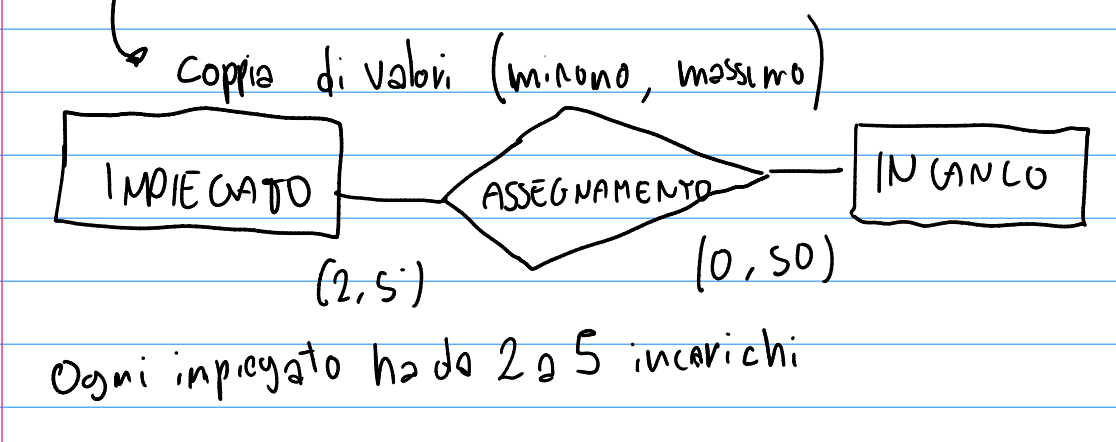
\includegraphics[width = \textwidth]{img/cardinalita_relazioni.png}

solitamente si usano numeri o identificatori come 0,1,n.

Posso definire cardinalità anche relativamente agli attributi.

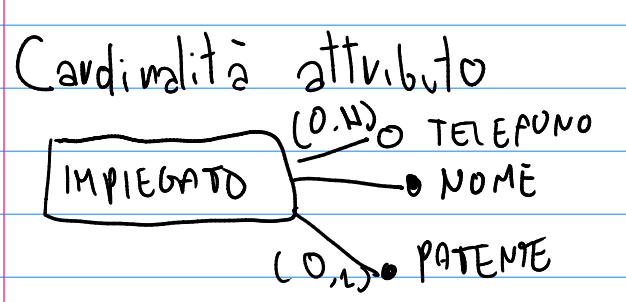
\includegraphics[]{img/cardinalita_attributi.png}

\subsection{Le relazioni}

Esistono vari tipi di relazioni:
\begin{itemize}
    \item binarie
    \item n-arie
    \item ricorsive
\end{itemize}

\paragraph{Relazioni binarie} Una relazione è binaria quando si rapporta a due entità e ne definisce un rapporto.

\paragraph{Relazioni n-arie} Se ho una relazione tra tre\footnote{Ad esempio in questo caso è ternaria} o più entità la relazione sarà n-aria. Un esempio di relazione ternaria è se ad esempio do due volte lo stesso esame avrò tre entità: \textit{persona}, \textit{esame1}, \textit{esame2}

\paragraph{Relazioni ricorsive} Posso avere relazioni ricorsive in molti casi, ad esempio se ho un prodotto che può essere composto da più prodotti ho una relazione ricorsiva con l'entità \textit{prodotto}.

\subsubsection{Gli attributi}

Gli attributi descrivono un' entità. Nel diagramma ER si definiscono con due simboli:

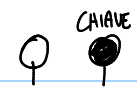
\includegraphics{img/attributi.png}

Il simbolo vuoto indica un'attributo normale, un attributo pieno indica un attributo chiave.

\paragraph{Gli attributi chiave} Un attributo chiave è un attributo che identifica in maniera univoca un oggetto appartenente a quell'entità. Per un cittadino italiano la chiave è il codice fiscale e ogni cittadino è identificato da questa chiave.

\paragraph{Attributi composti} Oltre agli attributi singoli descrivibili semplicemente con il simbolo vuoto posso anche voler descrivere attributi composti, ad esempio un indirizzo è un attributo composto da: Via, numero, cap, città, ecc...


\subsection{Design patterns}
Questi sono alcuni dei design patterns più utilizzati quando si organizza uno schema ER. Questi pattern sono comodi perchè semplificano la creazione e la lettura di un ER graph.

\subsubsection{Reificazione di attributo di entità}
Reificare significa prendere l'astratto per concreto, ovvero considerare concetti, categorie, idee, rapporti astratti alla stregua di oggetti concreti.

In questo caso significa espandere un attributo trasformandolo in entità. Questo è comodo perché ci consente di dare all'attributo altri sotto attributi e in caso di bisogno lo si potrà anche mettere in relazione con altre entità.
\begin{center}
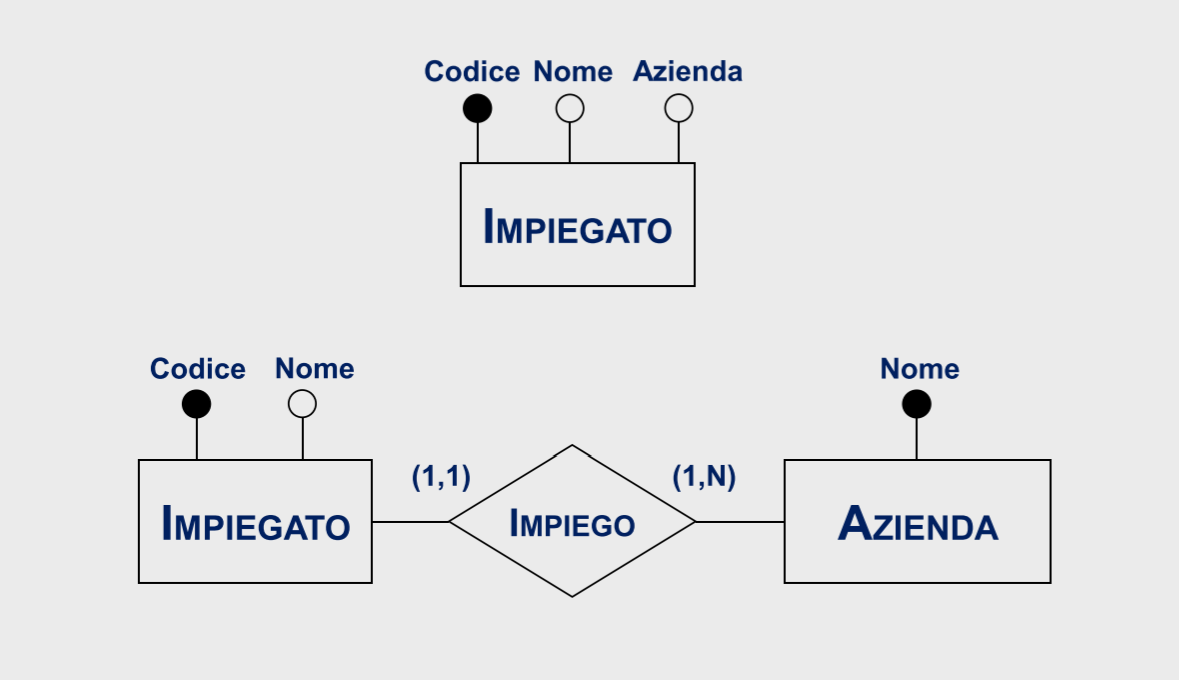
\includegraphics[width=0.5\textwidth]{img/reificazioneDiAttributoDiEntita.png}
\end{center}

\subsubsection{Part-of (Has-a)}
Quando un'entità non può esistere senza una sua sovra-entità, questa entità è "\textit{part-of}" della sovra-entità.

\begin{center}
    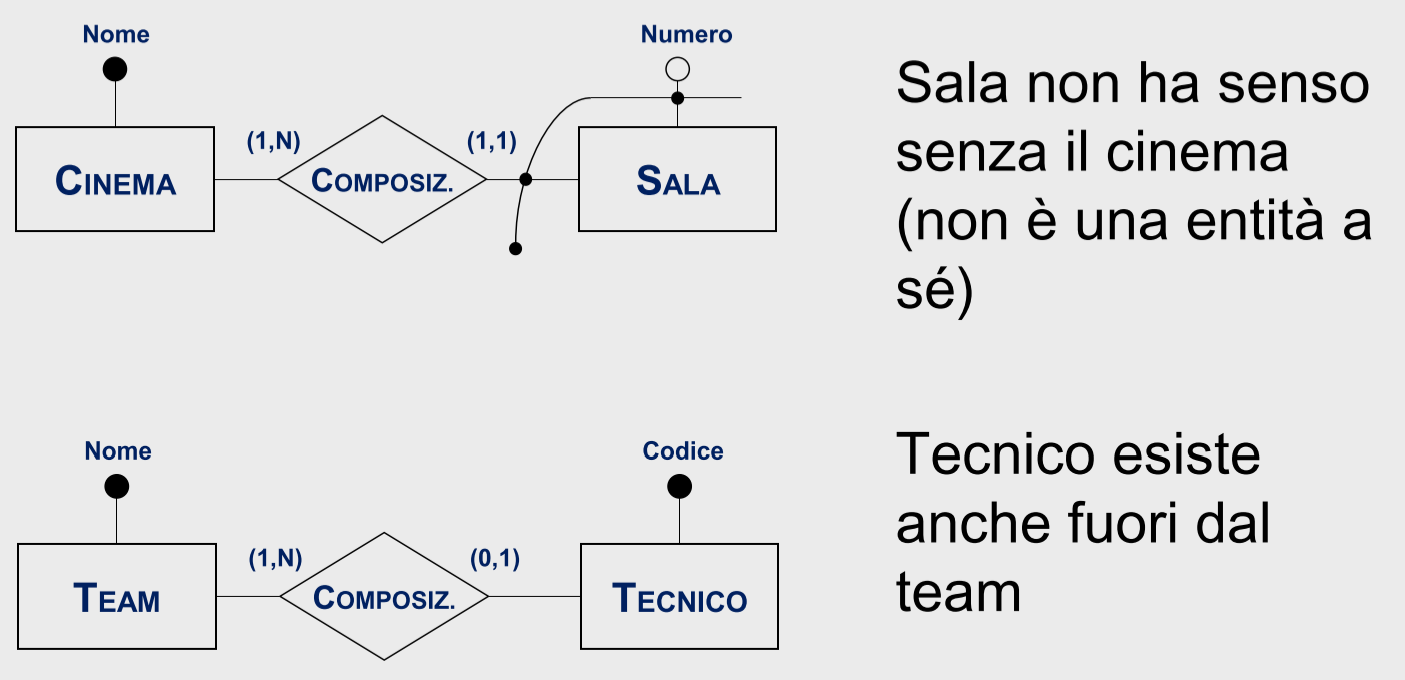
\includegraphics[width=0.7\textwidth]{img/partOf.png}
\end{center}

\subsubsection{Istance-of - Is-a}

Quando un'entità è una specifica versione di un'altra entità è un "\textit{Istance-of}" dell'altra entità.

\begin{center}
    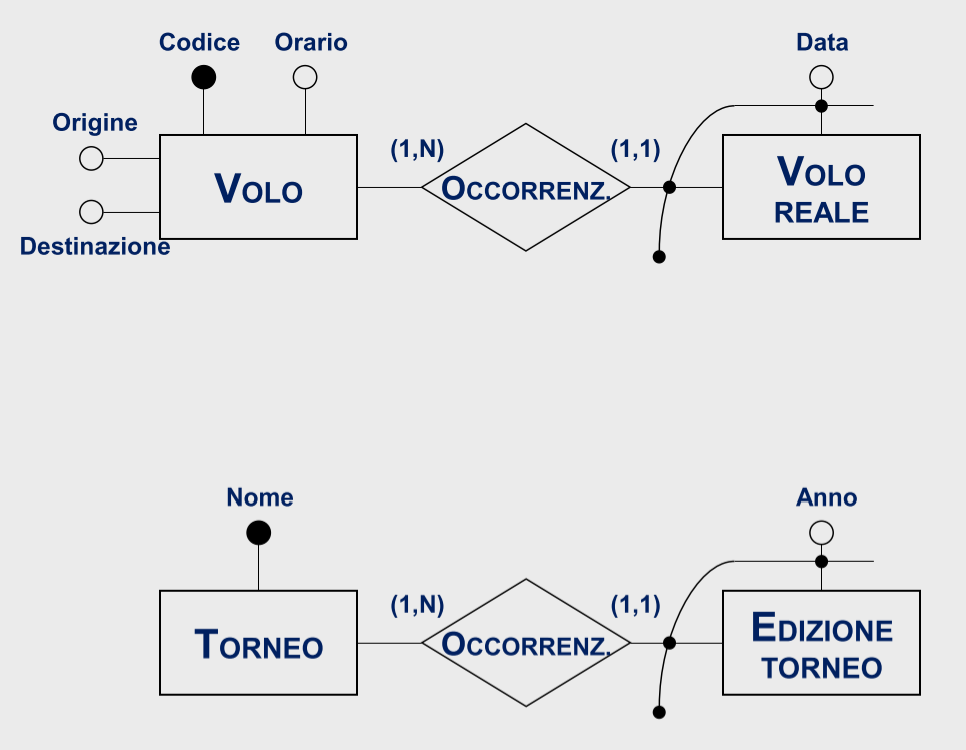
\includegraphics[width=0.7\textwidth]{img/istanceOf.png}
\end{center}

\subsubsection{Reificazione di relazione binaria}

\begin{center}
    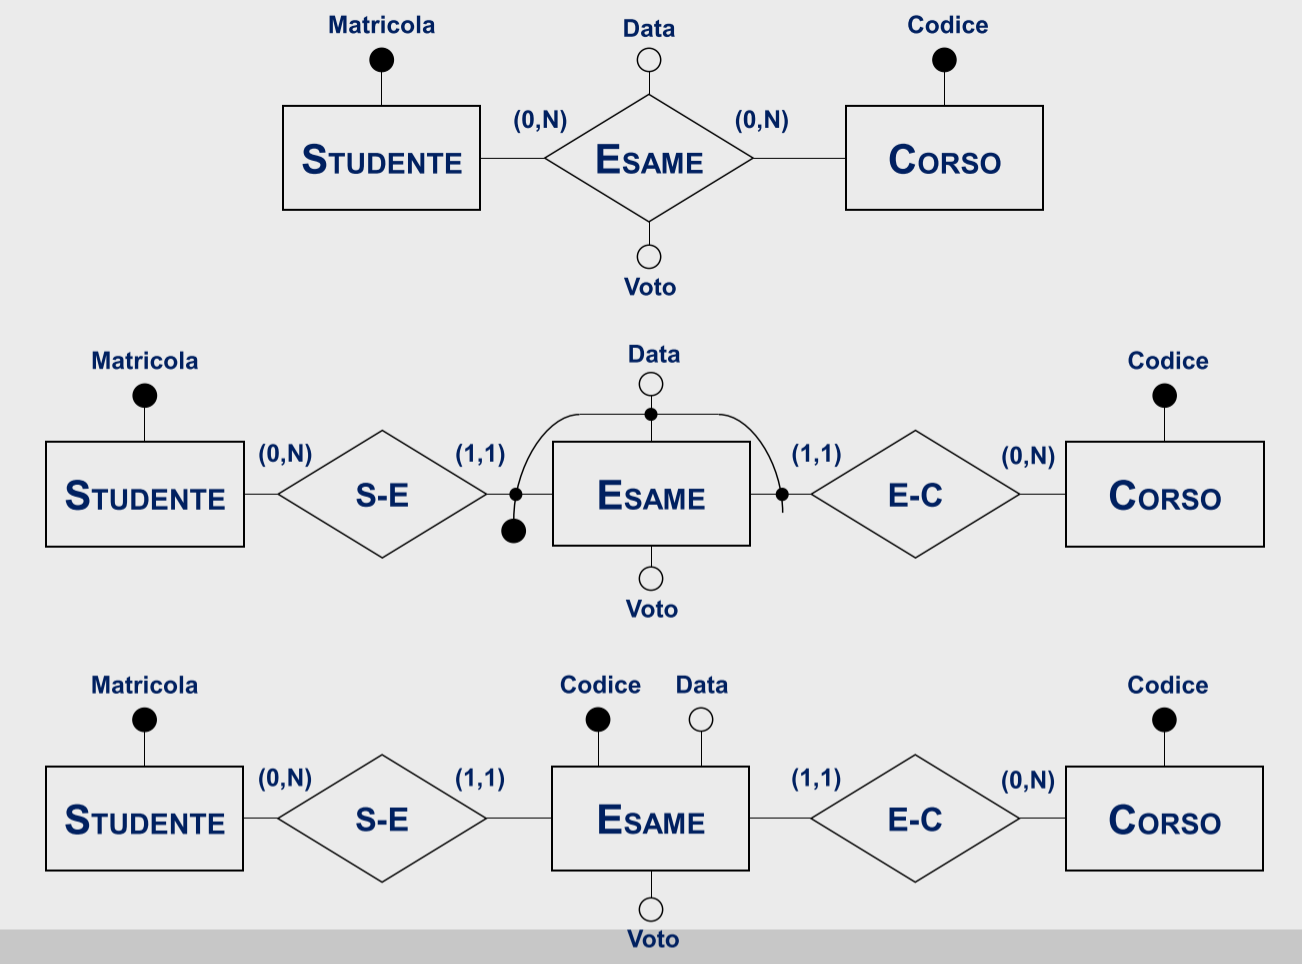
\includegraphics[width=0.7\textwidth]{img/reificazioneDiRelazioneBinaria.png}
\end{center}

\subsubsection{Reificazione di relazione ricorsiva}

\begin{center}
    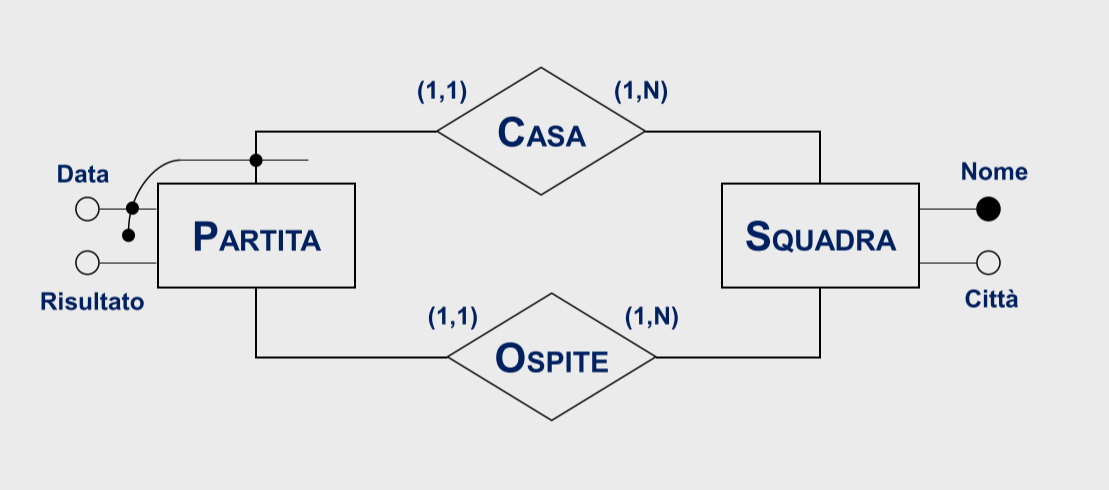
\includegraphics[width=0.7\textwidth]{img/reificazioneDiRelazioneRicorsiva.png}
\end{center}


\subsubsection{Reificazione di attributo di relazione}

\begin{center}
    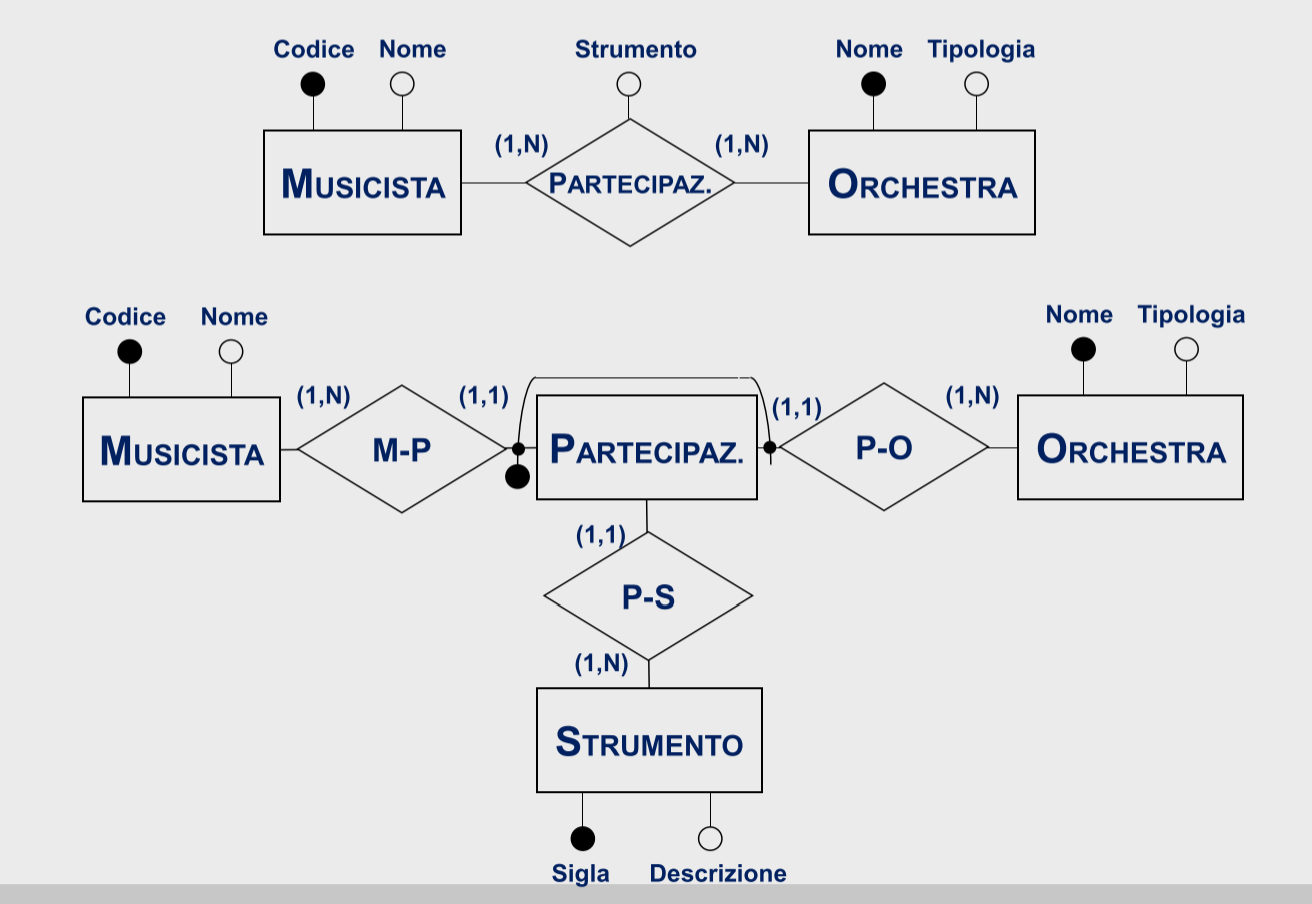
\includegraphics[width=0.7\textwidth]{img/reificazioneDiAttributoDiRelazione.png}
\end{center}

\subsubsection{Caso particolare}


\begin{center}
    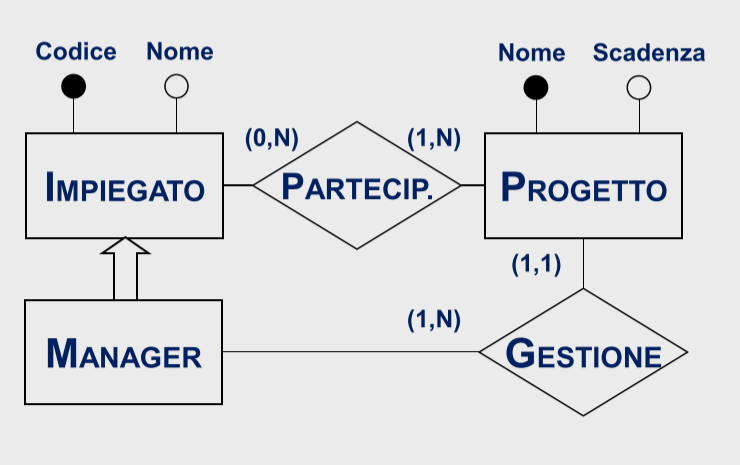
\includegraphics[width=0.7\textwidth]{img/casoParticolare.png}
\end{center}
\subsubsection{Storicizzazione di un concetto}

\begin{center}
    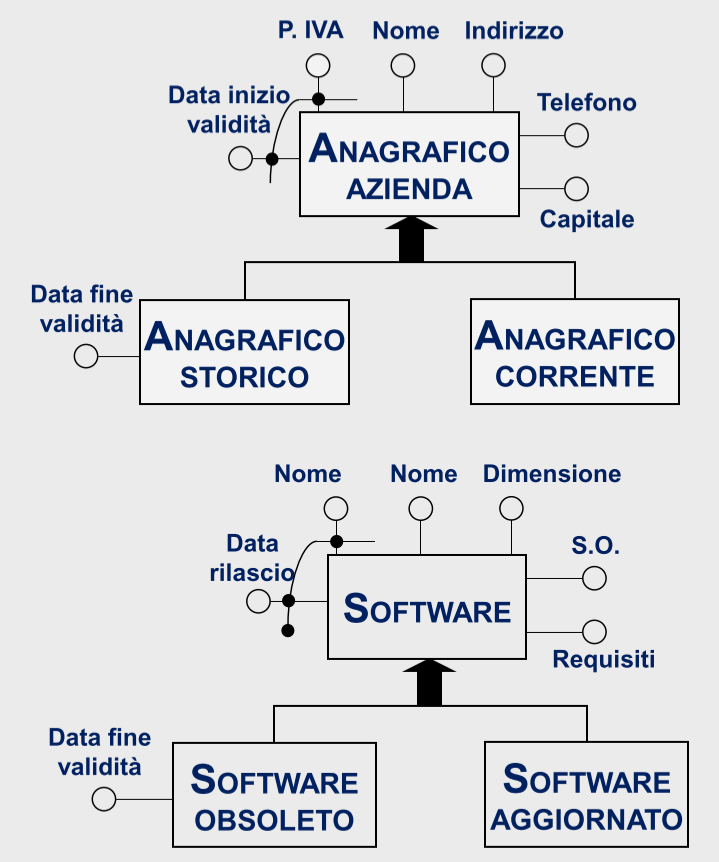
\includegraphics[width=0.7\textwidth]{img/storicizzazioneDiConcetto.png}
    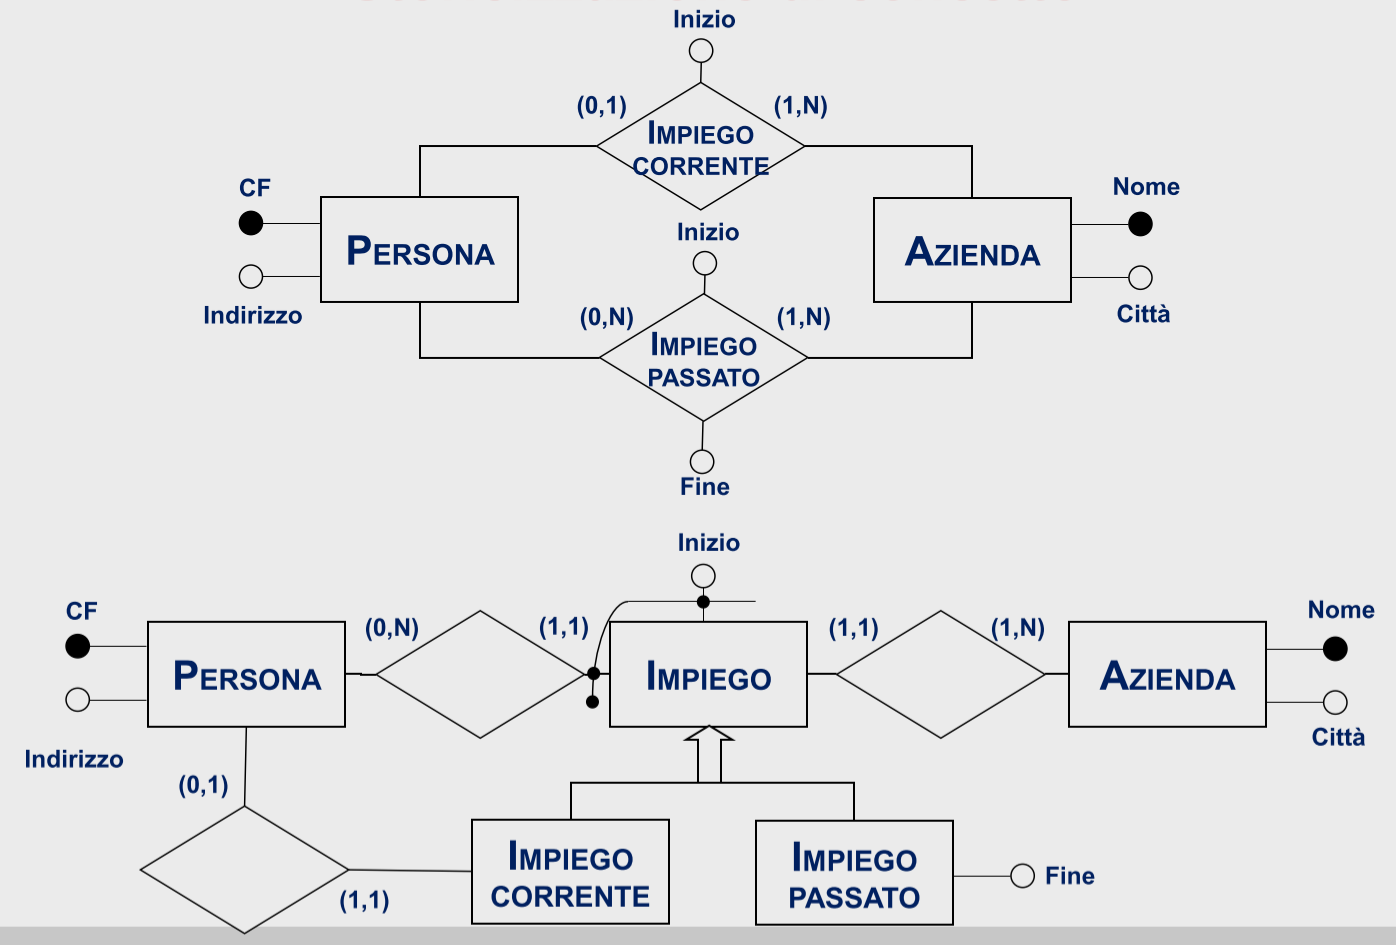
\includegraphics[width=0.7\textwidth]{img/storicizzazioneDiConcetto2.png}
\end{center}

\subsubsection{Evoluzione di un concetto}

\begin{center}
    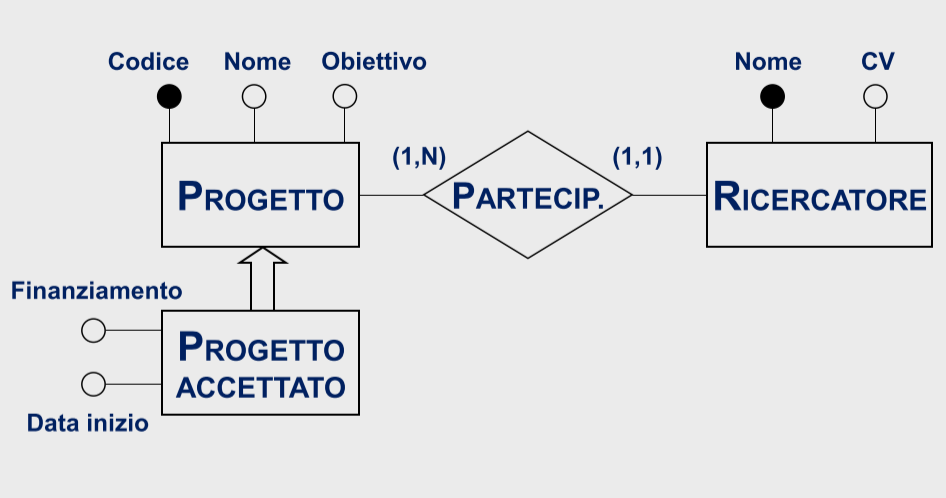
\includegraphics[width=0.7\textwidth]{img/evoluzioneDiConcetto.png}
\end{center}

\subsubsection{Relazione ternaria}

\begin{center}
    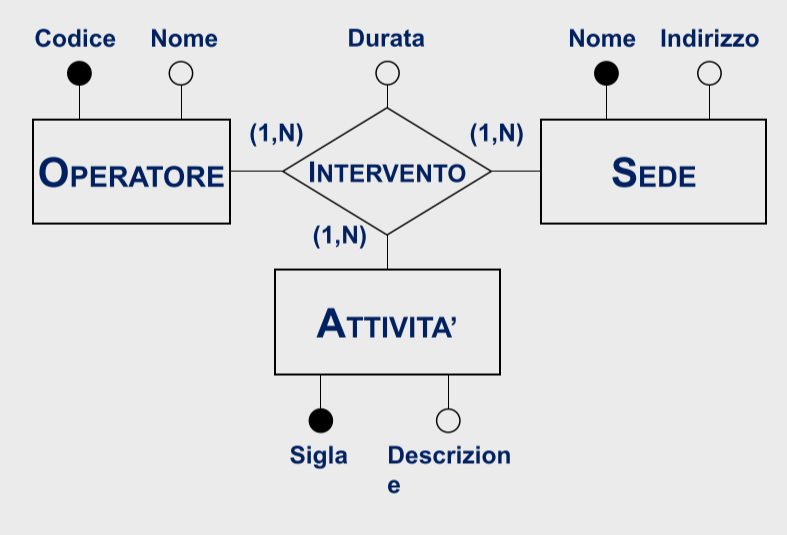
\includegraphics[width=0.7\textwidth]{img/relazioneTernaria.png}
\end{center}

\subsubsection{Reificazione di relazione ternaria}
\begin{center}
    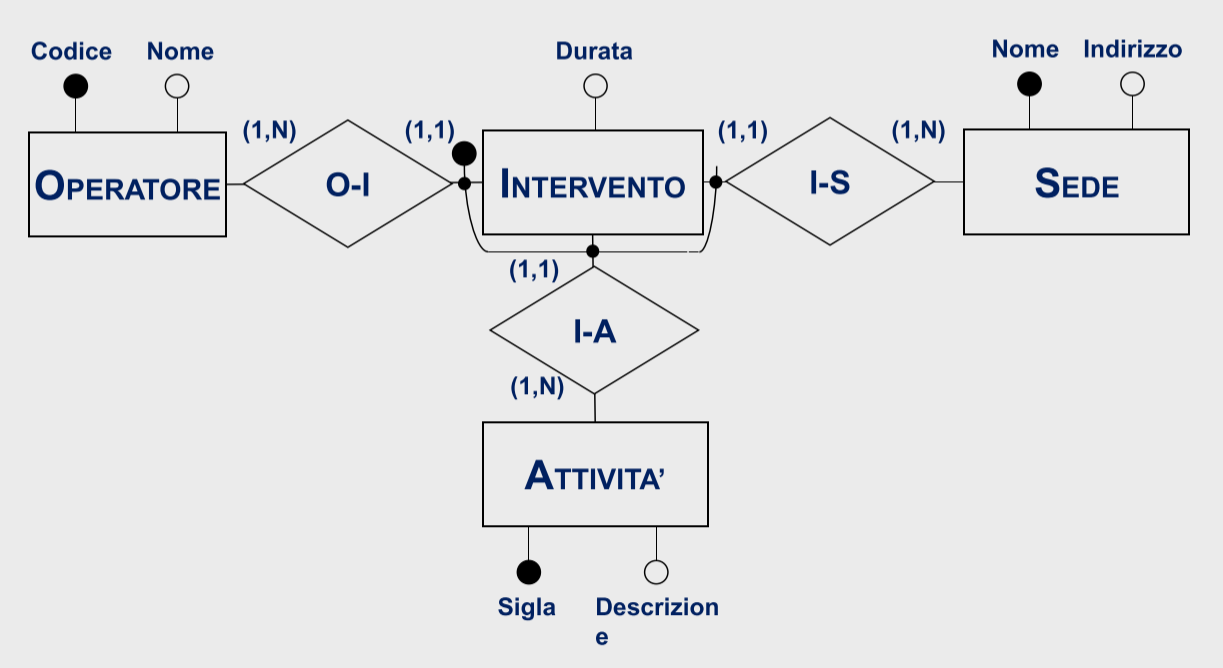
\includegraphics[width=0.7\textwidth]{img/reificazioneDiRelazioneTernaria.png}
    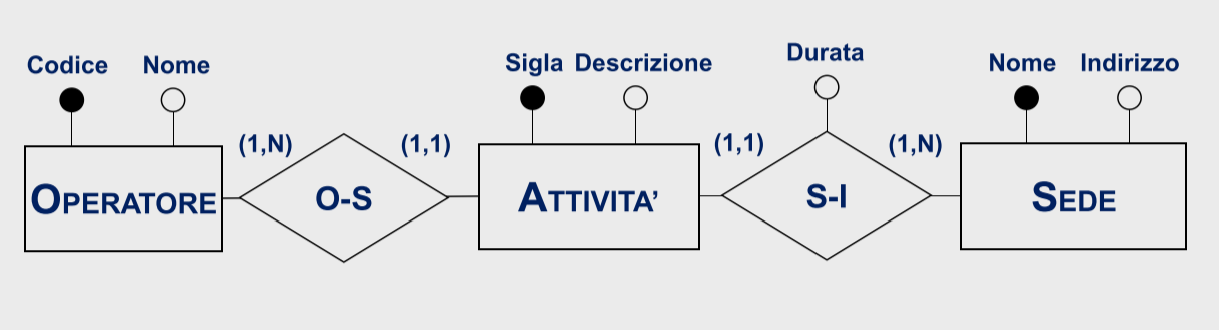
\includegraphics[width=0.7\textwidth]{img/reificazioneDiRelazioneTernaria2.png}
\end{center}

\section{Analisi}

Durante questa fase, lo scopo è quello di comprendere al meglio e nella maniera più aderente possibile cosa si dovrà modellare poi nelle fasi successive. I passaggi sono inquadrati nel seguente modo:

\begin{enumerate}
    \item Acquisizione dei requisiti
    \item Analisi dei requisiti
    \item Costruzione dello schema concettuale
    \item Costruzione del glossario
\end{enumerate}

In questa fase devo quindi acquisire i requisiti per la realizzazione, analizzare i dati raccolti e dovrò da queste informazioni ottenute generare uno schema relazionale ed un glossario dei termini.

\subsection{Acquisizione dei requisiti}

Questo è il momento in cui dovrò ascoltare utenti e committenti attraverso interviste o attraverso la lettura di documentazione precedentemente redatta.

Esempi di documenti da analizzare sono realizzazioni preesistenti e procedure aziendali.

Inoltre è poi importante controllare fonti, documentazioni, leggi e regolamenti.

Il reperimento dei requisiti è un'attività critica, complessa e non standardizzabile. Esistono però delle regole generali che conviene seguire.

\begin{itemize}
    \item Scegliere il corretto livello di astrazione
    \item Standardizzare la struttura delle frasi
    \item Suddividere le frasi articolare
    \item Separare le frasi sui dati da quelle sulle funzioni
    \item Costruire un glossario dei termini
    \item Individuare omonimi e sinonimi
    \item Rendere esplicito il rifermento tra termini
    \item Riorganizzare le frasi per concetti
\end{itemize}



\subsection{Progettazione concettuale}

È importante iniziare da una progettazione concettuale e quindi da uno schema concettuale poiché è importante avere a mente e chiarire in maniera solida e visiva quelli che sono i concetti che dovremo memorizzare nella base dati.

Se iniziassimo subito a mettere mano alle componenti specifiche delle basi di dati sarebbe difficile capire da dove iniziare e si rischierebbe di perdersi, infatti il modello logico ha molto focus sui dati e la rappresentazione delle relazioni e delle classi.

Il modello concettuale serve a ragionare sulla realtà di interesse indipendentemente dagli aspetti realizzativi. Questo ci permette di visualizzare quella che è la realtà in maniera schematica e chiara.

Il modello concettuale permette di rappresentare le classi di oggetti di interesse e le loro correlazioni.

Lo schema che utilizzeremo per rappresentare il modello sarà uno schema \textbf{ER}\footnote{Entità Relazione}.

\chapter{Generalizzazioni}

Una generalizzazione è il processo attraverso il quale viene associato ad una varietà di elementi il medesimo significato. Con generalizzazione viene indicato anche il significato ottenuto attraverso questo processo. Con generalizzazione viene indicato sia il processo cognitivo che la conoscenza risultante da questo processo. La generalizzazione ha la funzione di attenuare una varietà degli elementi allo scopo di semplificarne la gestione.

\begin{exmp}
Un esempio esplicativo di questa situazione può essere un esempio relativo agli alberi.

Un olmo, un oleandro, un pesco, un albicocco si possono tutti generalizzare in "\textbf{Un albero}"
\end{exmp}

Matematicamente parlando, considerando $E$ generalizzazione ogni proprietà di $E$ è anche proprietà di $E_1, ... E_n$ oggetti superiori.

Ogni istanza degli oggetti superiori $E_1, ..., E_n$ è istanza di $E$ generalizazzione.

Esistono vari tipi di generalizzazioni che differiscono a seconda della complessità e aderenza tra sovraoggetti e genralizzazione.

\begin{description}
	\item[N.B.] È importante ricordare che posso avere più tipi di generalizzazioni assieme e contemporaneamente.
\end{description}


\section{Generalizzazione totale e parziale}
\subsection{Totale}
Ogni occorrenza di $E$  è anche uno tra $E_1, ..., E_n$

\begin{exmp}
 "\textbf{una persona}"
\end{exmp}

In questo tipo di generalizzazione, se \textbf{sommiamo tutti i sovra-oggetti otteniamo l'insieme completo} della generalizzazione.

Nella rappresentazione ER, una generalizzazione di questo tipo è definita con una freccia grande dal corpo pieno(solitamente nero).

\subsection{Parziale}

In questo tipo di generalizzazione se sommiamo tutti i sovra-oggetti \textbf{non} otteniamo l'insieme completo della generalizzazione
Non tutte le $E$ sono un $E_1, ..., E_n$

\begin{exmp}
Un dottore e un avvocato possono essere generalizzati in "\textbf{una persona"}, però le persone non sono tutte avvocati o dottori.
\end{exmp}

\section{Generalizzazioni esclusive e sovrapposte}

Una generalizzazione è esclusiva quando l'intersezione dei figli è vuota.

Le generalizzazioni esclusive sono le più semplici ed in ogni caso si può semplicemente passare da una generalizzazione sovrapposta ad una generalizzazione esclusiva semplicemente dividendo la generalizzazione sovrapposta in più generalizzazioni esclusive che alla bisogna possono diventare parziali.

Una generalizzazione è sovrapposta quando l'intersezione dei figli \textbf{non} è vuota
\begin{exmp}
    Un \textit{Cliente} e un \textit{Venditore} sono entrambe \textbf{Persone} ma una \textbf{persona} può essere sia un cliente che un venditore.
\end{exmp}

\section{Conclusioni}

Concludendo, una generalizzazione può essere di questi 4 tipi ovvero combinazioni delle precedenti.

\begin{itemize}
    \item totale esclusiva
    \item totale sovrapposta
    \item parziale esclusiva
    \item parziale sovrapposta
\end{itemize}
\chapter{Normalizzazione}

La normalizzazione è un processo utilizzato per trasformare una base di dati non progettata in maniera corretta in una che sia tale.

La normalizzazione si può inoltre usare per capire se la progettazione effettuata è stata corretta.

\section{Anomailie}

Se una base di dati non è normalizzata possono sussistere varie anomalie che possono precludere la consistenza e la solidità di una base di dati.

\begin{itemize}
    \item Ridondanza
    \item Anomalia di aggiornamento
    \item Anomalia di cancellazione
    \item Anomailia di inserimento
\end{itemize}

\paragraph{Ridondanza}
Ho che uno stesso dato viene ripetuto più volte nella tabella.

\paragraph{Anomalia di aggiornamento}
Se un dato ridondante varia è necessario che quella ridondanza venga manuta consistente in tutte le tuple uguali. Altrimenti rischio inconsistenze che non sono facilmente gestibili.

\paragraph{Anomalia di cancellazione}
Se cancello una tupla e a quella tupla sono legate delle informazioni che non vorrei cancellare ma che essendo costruita male la struttura della tabella devo cancellare, ho perdita di dati.

\paragraph{Anomalia di inserimento}
Se ho un dato da voler inserire che non conosce gli altri campi dati della tupla non posso inserirlo perchè mancano delle informazioni che non posso avere.

In poche parole queste anomalie derivano dal fatto che in una stessa tabella sono state aggiunte troppe informazioni e non viene rispettato il principio della singola responsabilità.

\section{Dipendenze funzionali}

Una base di dati avrà sempre intrinsecamente delle dipendenze funzionali, queste dipendenze definiscono che se A avrà un certo valore allora B avrà sempre un valore relativamente ad A

\[ A \rightarrow B\]

\begin{exmp}
    $\text{Impiegato} \rightarrow \text{Stipendio}$
\end{exmp} 

Se ho una dipendenza funzionale gestita in maniera non corretta avrò una delle anomalie precedentemente descritte.

Matematicamente una dipendenza funzionale è definita come:

\[\forall t_1,t_2 \in R(X) : \pi_Y(t_1) = \pi_Y(t_2) \implies \pi_Z(t_1) = \pi_Z(t_1) \]

%Le dipendenze migliori sono quelle dove la parte di sinistra è superchiave della relazione.

Una dipendenza funzionale buona non causa anomalie.

Infatti, se la dipendenza funzionale ha a sinistra della dipendenza una chiave, allora nella parte destra avrò un dato che è responsabilità della tabella immagazzinare. Questo viene però definito in maniera più completa nelle forme normali.

\subsection{Copertura ridotta}

Una copertura ridotta è quando, per comprendere meglio le dipendenze funzionali, si scompongono le dipendenze al loro minimo.

Per estrarre la copertura ridotta, in una dipendenza funzionale, al lato destro della frecca deve essere presente un solo attributo.

\begin{exmp}
    Avendo una dipendenza funzionale del tipo:

    \[M \rightarrow RSDG\]

    Posso scomporla in:

    \[M \rightarrow R, M \rightarrow S,M \rightarrow D,M \rightarrow G\]

\end{exmp}



\section{Forme normali}

Le forme normali definiscono un pattern per strutturare la gestione delle dipendenze funzionali in modo da evitare le anomalie.

\subsection{Forma normale di Boyce Codd(BCNFF)}

Una relazione è in forma normale di BC se ogni dipendenza funzionale non banale è buona.

Questa forma normale da inoltre uno strumento per rendere una relazione priva di anomalie.

Per ogni dipendenza xy che viola bcnf creo una relazione xy e tolgo y dalla tabella di partenza.

\subsection{Terza forma normale}

La terza forma normale da delle condizioni meno stringenti rispetto alla forma normale di Boice Codd.

\subsection{Svolgere gli esercizi}

\begin{exmp}
    Data la relazione 
    \[R(A,B,C,D)\]
    Con dipendenze funzionali
    \[ C \rightarrow D,C \rightarrow A,B \rightarrow C \]
    
    \begin{enumerate}
        \item Mostrare tutte le chiavi di R e motivare perché ognuna è chiave.
        \item Dire quali dipendenze violano la forma normale di Boyce Codd spiegandone la ragione.
        \item Decomporre in BCNF
    \end{enumerate}
    
    \paragraph{1.} Per trovare le chiavi dobbiamo per prima cosa calcolare le chiusure, sicuramente andremo a calcolare le chiusure di tutte le parti sinistre delle dipendenze. ovvero C e B

    Calcolare le chiusure significa cercare relativamente ad ogni attributo dove si può andare a finire seguendo le frecce.

    \begin{equation} \label{eq1}
        \begin{split}
            C^+&= \left\{ C \right\} \\
            &= \left\{ C,D \right\}  \\
            &= \left\{ C,D,A \right\}  \\
        \end{split}
    \end{equation}

    Quindi qui ad esempio da C potevamo andare in A e da C potevamo andare in d

    \begin{equation} \label{eq1}
        \begin{split}
            B^+&= \left\{  B \right\}\\
            &= \left\{  B,C \right\}\\
            &= \left\{  B,C,D \right\}\\
            &= \left\{  B,C,D,A \right\}\\
        \end{split}
    \end{equation}

    Nella chiusura qui sopra invece da B siamo andati in C e da C potevamo percorrere tutte le strade della ciusura di C.

    Come risultato di questi calcoli otteniamo quindi le due chiusure.

    \[C^+= \left\{ C,D,A \right\} \] \[ B^+= \left\{  B,C,D,A \right\}\]

    Ci accorgiamo che la chiusura di \textbf{B} contiene tutti gli attributi della relazione. Per questo motivo possiamo quindi dire che B è chiave della relazione.

    \paragraph{2.}

    Pe trovare quali dipendenze violano la forma normale BCNF dobbiamo controllare quali di queste dipendenze non hanno una superchiave\footnote{Le dipendenze che rispettano la BCNF sono solo le dipendenze "Buone"} al lato sinistro della rappresentazione.

    in questo caso la nostra chiave e superchiave è $B$. 

    Possiamo quindi notare come $C \rightarrow D$ e $C \rightarrow A$ violino BCNF dato che C non è superchiave.

    Siccome abbiamo delle violazioni di BCNF dobbiamo trovare come decomporre la relazione tramite BCNF.

    \paragraph{3.} Per decomporre in BCNF dobbiamo estrarre dalla relazione tutti quegli attributi che rischiano di essere interessati dalle anomalie.

    La decomposizione inizia togliendo la parte destra delle dipendenze funzionali dove l'attributo di sinistra non è chiave.

    Abbiamo quindi che la nostra relazione $R(A,B,C,D)$ con chiave trovata prima in $B$ viene separata in
    \[R(A,\underline{B},C) , R_1(\underline{C},D)\]

    Rimuoviamo poi la seconda dipendenza funzionale e ci troviamo nella situazione:

    \[R(\underline{B},C) , R_1(\underline{C},D), R_2(\underline{C},A)\]

    Possiamo quindi accorpare $R_1,R_2$ poichè hanno la stessa chiave e la situazione finale diventa:

    \[R(\underline{B},C), R_1(\underline{C},D,A)\]

\end{exmp}

\begin{exmp}
    Considerando lo schema relazionale $R(E,N,L,C,S,D,M,P,A)$ con le seguenti dipendenze funzionali ne calcoliamo una copertura ridotta e scomponiamo la relazione in terza forma normale.

    \[E \rightarrow NS, NL \rightarrow EMD, EN \rightarrow LCD, C \rightarrow S, D \rightarrow M, M \rightarrow D, EPD \rightarrow A, NLCP \rightarrow A\]

    \paragraph{La copertura ridotta}
    Scoponiamo allora in una copertura ridotta le precedenti dipendenze funzionali. Per prima cosa espandiamo i secondi membri delle dipendenze in più dipendenze.
    \[
    E \rightarrow N,
    E \rightarrow S,
    NL \rightarrow E,
    NL \rightarrow M,
    NL \rightarrow D,
    EN \rightarrow L,
    \]
    \[
    EN \rightarrow C,
    EN \rightarrow D,
    C \rightarrow S,
    D \rightarrow M,
    M \rightarrow D,
    EPD \rightarrow A,
    NLCP \rightarrow A
    \]

    Possiamo quindi rimuovere tutte le dipendenze eliminabili dal primo membro.

    Per fare questo dobbiamo vedere se ci sono dipendenze funzionali che possono essere usate per ridurre gli attributi al primo membro.

    In questo caso $EN$ presente al primo membro di $ EN \rightarrow L,
    EN \rightarrow C,
    EN \rightarrow D$ si trasforma in solo $E$

    Viene ridotto anche $EPD \rightarrow A $ in $ EP \rightarrow A$ utilizzando la dipendenza appena creatasi $E \rightarrow D$

    La terza e ultima riduzione è quella di $ NLCP \rightarrow A$ che viene ridotta in $NLP \rightarrow A $ utilizzando le dipendenze concatenate $NL \rightarrow E \rightarrow C$ 

    Otteniamo quindi il seguente risultato.

    \[
    E \rightarrow N,
    E \rightarrow S,
    NL \rightarrow E,
    NL \rightarrow M,
    NL \rightarrow D,
    E \rightarrow L,
    \]
    \[
    E \rightarrow C,
    E \rightarrow D,
    C \rightarrow S,
    D \rightarrow M,
    M \rightarrow D,
    EP \rightarrow A,
    NLP \rightarrow A
    \]

    Possiamo ora rimuovere le dipendenze ridondanti.

    Infatti ripercorrendo all'indietro le dipendenze possiamo vedere come $E \rightarrow S$ sia deducibile da $E \rightarrow C  \rightarrow S$.

    Anche $NL \rightarrow M$ è deducibile da $ NL \rightarrow E \rightarrow D \rightarrow M$.

    Un altro è $NL \rightarrow D$ deducibile da $NL \rightarrow E \rightarrow D $ 

    Risulta quindi:

    \[
        E \rightarrow N,
        NL \rightarrow E,
        E \rightarrow L,
        E \rightarrow C,
        E \rightarrow D,
        \]
        \[
        C \rightarrow S,
        D \rightarrow M,
        M \rightarrow D,
        NLP \rightarrow A
        \]

    Abbiamo quindi ottenuto la \textbf{Copertura ridotta}

    \paragraph{Le chiusure}

    Calcoliamo le chiusure di tutti i primi membri delle dipendenze

    \begin{equation}
        \begin{split}
            E^+&= \left\{E, N,L,C,D  \right\} \\
            &= \left\{ N,L,C,D,E,S,M, \right\}  \\
            &= \left\{ N,L,C,D,E,S,M,D \right\}  \\
        \end{split}
    \end{equation}

    \begin{equation}
        \begin{split}
            NL^+&= \left\{ N,L,E \right\} \\
            &= \left\{N,L,E, E^+ \right\}  \\
            &= \left\{ E,N,L,C,D,E,S,M,D\right\}  \\
        \end{split}
    \end{equation}
    \begin{equation}
        \begin{split}
            C^+&= \left\{C, S \right\} \\
        \end{split}
    \end{equation}
    \begin{equation}
        \begin{split}
            D^+&= \left\{D,  M\right\} \\
        \end{split}
    \end{equation}
    \begin{equation}
        \begin{split}
            M^+&= \left\{M, D \right\} \\
        \end{split}
    \end{equation}
    \begin{equation}
        \begin{split}
            NLP^+&= \left\{N,L,P,A, \right\} \\
            &= \left\{N,L,P,A,NL^+ \right\} \\
            &= \left\{N,L,P,A,NL^+ \right\} \\
            &= \left\{N,L,P,A,E,C,D,S,M \right\} \\
        \end{split}
    \end{equation}

    Notiamo che $NLP$ è superchiave ma la chiave migliore è la chiave più corta possibile.

    Sostituendo quindi $E$ ad $NL$ utilizzando la giusta dipendenza funzionale otteniamo che $EP$ è è la nostra chiave minimale.

    \paragraph{La decomposizione in BCNF}

    $R$ viene partizionato in sottoinsiemi tali che due dipendenze funzionali $X \rightarrow A$ e $Y \rightarrow B$ sono insieme se $X_G^+=Y_G^+$.

    In parole più semplici, se la chiusura di X e Y è la stessa esse sono in uno stesso insieme.

    \begin{equation}
        \begin{split}
            E^+ & = \left\{ N,L,C,D,E,S,M,D \right\}  \\
            NL^+ & = \left\{ N,L,C,D,E,S,M,D \right\}  \\
            C^+ & = \left\{C, S \right\} \\
            D^+ & = \left\{D,  M\right\} \\
            M^+ & = \left\{D,M \right\}  \\
            NLP^+ & = \left\{N,L,P,A,E,C,D,S,M \right\} \\
        \end{split}
    \end{equation}

    Dato che La chiusura di $E$ e di $NL$ sono le stesse posso racchiuderle in una sola relazione.

    Anche la chiusura di $D$ ed $M$

    Ottengo quindi le seguenti relazioni dove se esistono due relazioni $S(X)$ e $T(Y)$ con $X \subseteq Y$, $S$ viene eliminata

    \begin{equation}
        \begin{split}
            R_1 & =  (N,L,C,D,E ) \\
            R_2 & = (C, S)\\
            R_3 & = (D, M) \\
            R_4 & = (N,L,P,A) \\
        \end{split}
    \end{equation}
    Se, per qualche i, non esiste una relazione $S(X)$ con $K_i \subseteq X$, viene aggiunta una relazione $T(K_i )$.
    In parole povere se manca una relazione di collegamento tra le presenti questa relazione va creata.

    Dobbiamo quindi aggiungere $R_5 = (E,P)$
    
    \paragraph{Le chiavi}

    Notiamo quindi in fine le chiavi delle relazioni.

    \begin{equation}
        \begin{split}
            R_1 & = ( \underline{N,L},C,D,\underline{E}) \\
            R_2 & = (\underline{C}, S ) \\
            R_3 & = (\underline{D}, M) \\
            R_4 & = (\underline{N,L,P},A ) \\
            R_5 & = (\underline{E,P})\\
        \end{split}
    \end{equation}

    Abbiamo quindi completato l'esercizio.
\end{exmp}
\chapter{Gestione delle transazioni}

Le transazioni il paradigma utilizzato dai DBMS per gestire richieste concorrenti di lettura e scrittura sui dati.

Le transazioni sono suddivise principalmente in 3 parti:
\begin{itemize}
    \item Inizio della transazione
    \item Corpo di azioni della transazione
    \item Fine della transazione dove viene deciso se fare un commit della stessa oppure un rollback.
\end{itemize}

Un sistema transazionale è detto anche \textbf{OLTP} ed è in grado di definire ed eseguire transazioni per conto di un certo numero di applicazioni concorrenti. In parole più semplici offre un'interfaccia trasparente alle applicazioni mantenendo sicuro l'agire sui dati.

\begin{lstlisting}
start transaction;
update ContoCorrente
set Saldo = Saldo + 10 where NumConto = 12202;
update ContoCorrente
set Saldo = Saldo - 10 where NumConto = 42177;
commit work;
\end{lstlisting}

\section{ACID}

Abbiamo quindi che un'applicazione effettua molteplici transazioni e molte applicazioni effettuano parecchie transazioni in parallelo. Risulta importante per la base dati mantenere quindi il concetto di \textbf{ACID}

\textbf{ACID} é l'acronimo di:
\begin{itemize}
    \item Atomicity (Atomicità)
    \item Consistency (Consistenza)
    \item Isolation (Isolamento)
    \item Durability (Persistenza)
\end{itemize} 

Una transazione deve essere un'unità \textbf{atomica} di elaborazione. In parole semplici, o la transazione è fatta per intero oppure non deve essere eseguita per nulla.

\begin{exmp}
    L'esempio più classico di questa proprietà è quando si fa un movimento monetario in banca.
    
    Quando devo muovere del denaro da un conto ad un altro dovrò rimuovere del denaro da un primo conto e aggiungerlo in un secondo conto. Se per qualche malaugurato caso l'operazione non andasse a buon fine in un momento intermedio si rischierebbe di sballare i conteggi di uno dei due conti se non di entrambi.
    
    Cosa che per una banca può essere un problema di migliaia o milioni di euro.
\end{exmp}

Una transazione deve essere \textbf{Consistente}, deve infatti rispettare i vincoli imposti nella fase di progettazione del Database, come chiave, integrità referenziale, check, ecc.

Questi vincoli che determinano la consistenza dei dati vanno verificati solo a fine transazione, possono quindi essere violati temporaneamente nel mezzo di una transazione.

Se i vincoli risultano violati alla fine della transazione allora la transazione andrà in rollback.

Una transazione deve essere poi \textbf{Isolata}, non deve infatti risentire degli effetti delle altre transazioni concorrenti. In poche parole l'esecuzione concorrente deve produrre un risultato identico a quello che verrebbe ottenuto se le transazioni concorrenti venissero invece eseguite sequenzialmente.

Se una transazione esponesse i suoi stati intermedi si rischierebbe un effetto domino.

Gli effetti di una transazione che ha raggiunto il commit non devono essere persi in qualsiasi csao, anche in presenza di guasti.

Sia che questi guasti siano di dispositivo\footnote{Hardware} oppure che questi guasti siano di sistema\footnote{Software}.

\section{Processi di ripresa}

Le riprese da un crash sono di due tipi: ripresa a caldo e ripresa a freddo.

Una ripresa a freddo viene eseguita quando il problema è stato a livello Hardware, in quel caso si deve ripristinare i dati da un dump e in secondo luogo eseguire la ripresa a caldo.

La ripresa a caldo risolve tutti i problemi relativi alle transazioni in atto al momento del crash.

La ripresa a freddo si avvale di un dump eseguito periodicamente nel log. Il dump in oggetto viene copiato nel database e ne ripristina i dati fino al suo momento.

Dopo il dump bisognerà invece scorrere il log ed eseguire tutte le transazioni nella sequenza indicata.

\section{I vari schedule}

Uno schedule è una sequenza di operazioni di input/output concorrenti.

Lo \textbf{scheduler} invece è il sistema che accetta, rifiuta o riordina le operazioni richieste dalle transazioni.

Esistono vari tipi di \textbf{Scheduling} che ritornano vari tipi di schedule.

In uno schedule seriale le transazioni sono seprate e vengono eseguite una alla volta, questo tipo di schedule è sicuro perché eseguendo tutte le operazioni in ordine non è possibile trovarsi in una situazione di race condition. In tutti gli schedule successivi si cercherà infatti di tornare a questo tipo di schedule.

Avremo infatti uno \textbf{schedule serializzabile} quando uno schedule produce lo stesso risultato di uno schedule seriale eseguito sulle stesse transazioni.

\[ \text{Schedule seriale} \implies \text{Schedule serializzabile}\]

L'insieme degli schedule serializzabili contiene l'insieme degli schedule seriali.

Gli schedule serializzabili utilizzati sono:
\begin{itemize}
    \item View serializzabili
    \item Conflict serializzabili
    \item Two Phase locking
\end{itemize}

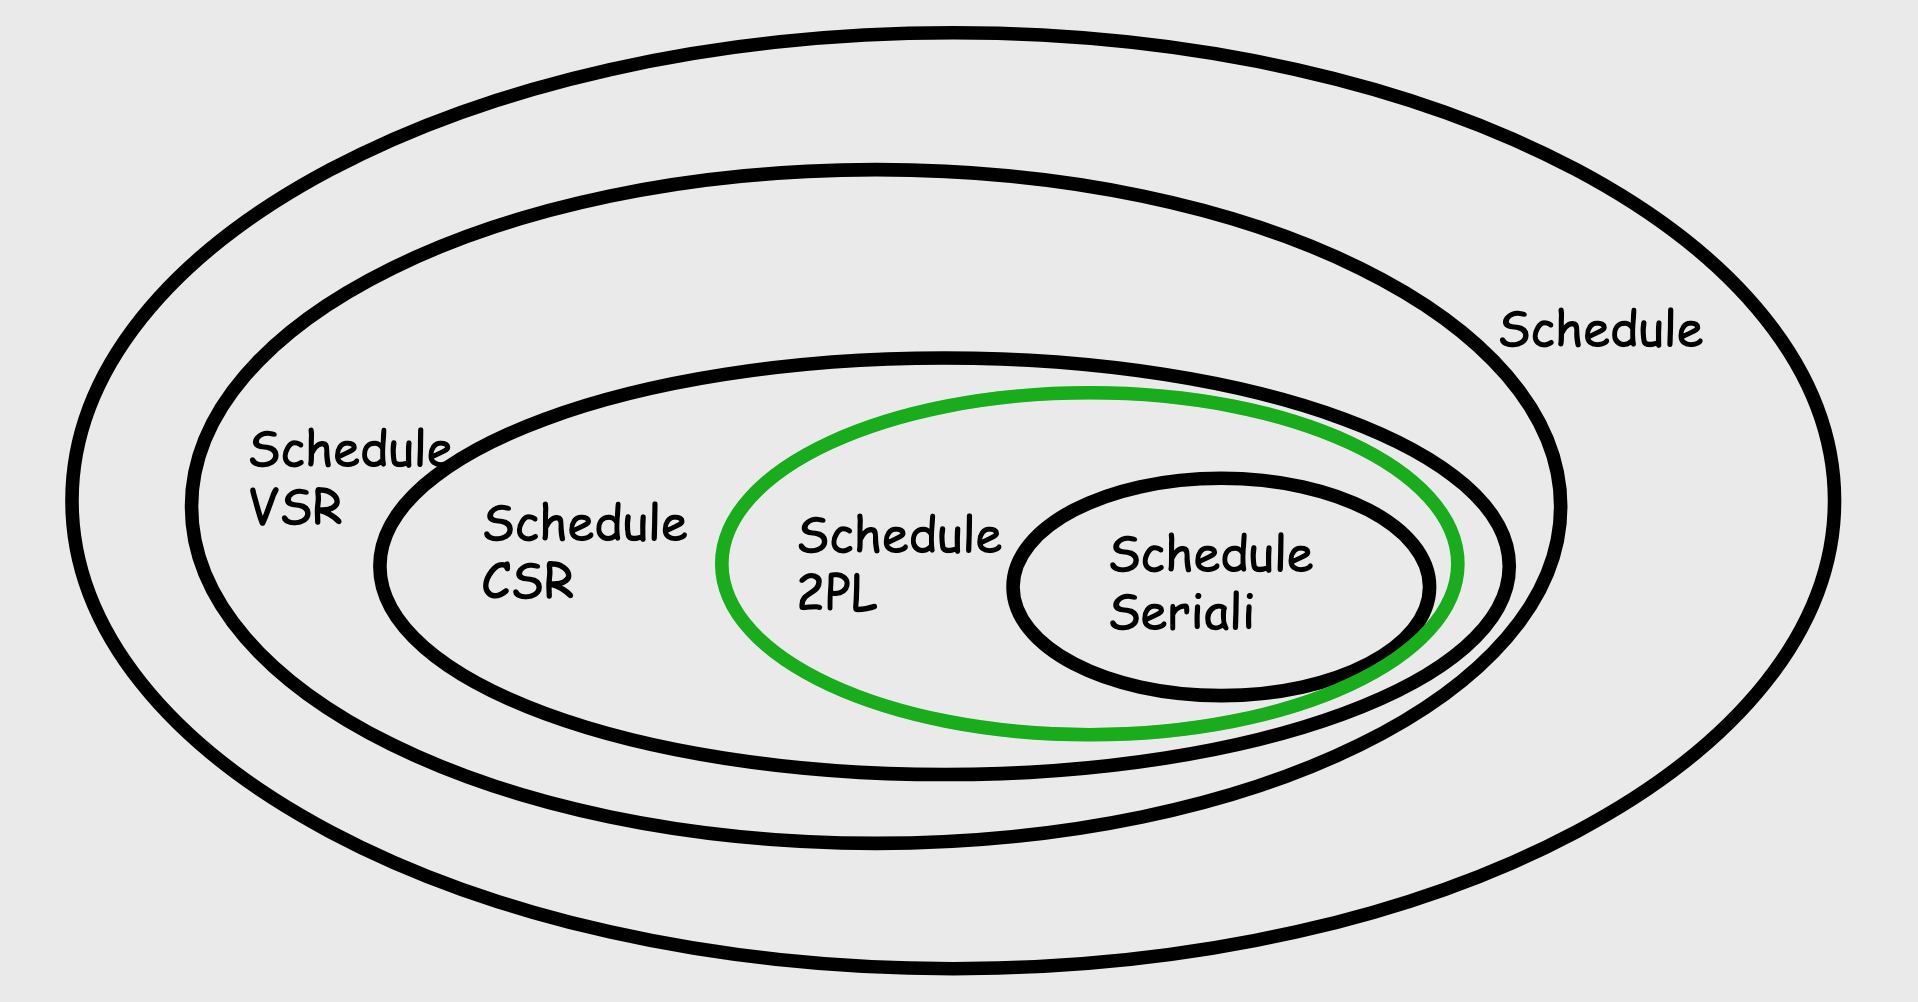
\includegraphics[width=\linewidth]{img/schedules.png}

\subsection{View serializzabilità}

Uno schedule è view serializzabile se è view equivalente ad almeno uno schedule seriale.

Uno schedule è view equivalente ad un altro se le letture leggono dagli stessi eventi come nell'altro schedule e la sequenza di scritture finali è la stessa.

Uno schedule view serializzabile offre numerose \textbf{garanzie}
\begin{itemize}
    \item Assienza di perdita di aggiornamento
    \item Assenza di letture inconsistenti
    \item Assenza di Gost updates
\end{itemize}

\subsection{Conflict serializzabilità}

Siccome cercare la view serializzabilità con molte transazioni diventa un lavoro molto costoso, si preferisce cercare la conflict serializzabilità. Si ha infatti che costa meno in tempo eseguire serialmente uno schedule view serializzabile ma non conflict serializzabile piuttosto che conoscere se esso è view serializzabile oppure no.

Se uno schedule è Conflict serializzabile allora è sicuramente anche View serializzabile. Uno schedule Conflict serializzabile è un sottoinsieme degli schedule View serializzabili.

\[CSR \implies VSR \implies \text{Schedule serializzabile}\]

Se uno schedule è conflict serializzabile allora è possibile costruire un grafo aciclico dei conflitti.

Infatti se abbiamo un grafo aciclico dei conflitti possiamo anche comprendere se il nostro schedule è conflict serializzabile. Inoltre il grafo ci può fornire anche un ordine in cui le transazioni devono essere eseguite per avere uno schedule seriale.

Un'azione $a_i$ è in conflitto con $a_j | (i \neq j)$, se operano sullo stesso
oggetto e almeno una di esse è una scrittura. Due casi:
\begin{itemize}
    \item conflitto read-write (rw o wr)
    \item conflitto write-write (ww)
\end{itemize}

Lo schedule seriale è conflict equivalente e quindi view equivalente. Ovvero posso trovare uno schedule conflict serializzabile, conflict equivalente ad uno schedule seriale.

\subsection{Svolgere gli esercizi}

Una raccolta di esercizi esemplificativi ed eseplicativi degli esercizi sugli schedule.
   

\begin{exmp}
    Dato lo schedule:

    \[S = r_1(x), w_2(x), r_3(x), w_1(u), w_3(v), r_3(y), r_2(y), w_3(u), w_4(t), w_3(t)\]

    Possiamo dire se è conflict serializzabile disegnando il grafo dei conflitti.

    Seguendo l'algoritmo scorriamo ognuno dei punti della serie di transazioni e vediamo se va in conflitto con una qualsiasi altra unità di transazione.

    Ad esempio, partendo da \textbf{$r_1$} che fa una lettura su \textbf{$x$}, vediamo che la stessa \textbf{$x$} è utilizzata in \textbf{$w_2$}. \textbf{$r_3$} non è in conflitto con \textbf{$r_1$} in quanto essendo due letture non ho problemi anche se l'accesso fosse simmultaneo.

    Disegnamo allora un vettore da dalla transazione 1 alla transazione 2.
    \begin{center}
        \begin{tikzpicture}[node distance={15mm}, main/.style = {draw, circle}] 
        
            \node[main] (1) {$t_1$}; 
            \node[main] (2) [above right of=1]{$t_2$}; 
            \node[main] (3) [below right of=1]{$t_3$}; 
            \node[main] (4) [above right of=3]{$t_4$};
            \draw[->] (1) -- (2);
        \end{tikzpicture} 
    \end{center}

    Continuando a seguire l'algoritmo per tutti gli altri punti il risultato è il seguente:
    \begin{center}
        \begin{tikzpicture}[node distance={15mm}, main/.style = {draw, circle}] 
        
            \node[main] (1) {$t_1$}; 
            \node[main] (2) [above right of=1]{$t_2$}; 
            \node[main] (3) [below right of=1]{$t_3$}; 
            \node[main] (4) [above right of=3]{$t_4$};
            \draw[->] (1) -- (2);
            \draw[->] (2) -- (3);
            \draw[->] (1) -- (3);
            \draw[->] (4) -- (3);
        \end{tikzpicture} 
    \end{center}

    Da questo grafo appena disegnato possiamo quindi estrarre uno Schedule seriale.

    Per prima cosa andranno tutte le transazioni senza vertici entranti, ovvero $t_1, t_4$ dopo questo l'algoritmo continua contando i nodi già estratti come senza vertici uscenti.

    Il risultato è quindi la sequenza $t_1 \rightarrow t_4 \rightarrow t_2 \rightarrow t_3$.
    
    Lo schedule seriale è quindi:

    
    \begin{center}
        \begin{tabularx}{10cm}{|p{25mm}|X|}
            \hline
            \rowcolor{gray!30}
            \textbf{Transazione} & \textbf{operazioni}\\
            \hline
            $t_1$& $r_1(x), w_1(u)$\\
            $t_4$& $w_4(t)$\\
            $t_2$& $w_2(x), r_2(y)$\\
            $t_3$& $r_3(x), w_3(v), r_3(y), w_3(u), w_3(t)$\\
            \hline
        \end{tabularx}
    \end{center}

    Che risulta nello schedule completo:
    \[S_\text{seriale} = r_1(x), w_1(u), w_4(t), w_2(x), r_2(y), r_3(x), w_3(v), r_3(y), w_3(u), w_3(t)\]

    Questo schedule seriale è \textbf{Conflict equivalente} allo schedule $S$ ed essendo \textbf{Conflict equivalente} è anche \textbf{View equivalente}.
\end{exmp}

\begin{exmp}
    Se abbiamo uno Schedule

    \[S = w_1(x), w_2(x), r_2(x), w_1(x)\]

    Possiamo vedere se è view equivalente confrontando tutte le permutazioni delle transazioni.

    Ovvero le seguenti transazioni:

    \begin{center}
        \begin{tabularx}{10cm}{|p{25mm}|X|}
            \hline
            \rowcolor{gray!30}
            \textbf{Transazione} & \textbf{operazioni}\\
            \hline
            $t_1$& $w_1(x), w_1(x)$\\
            $t_2$& $w_2(x), r_2(x)$\\
            \hline
        \end{tabularx}
    \end{center}

    Possiamo ordinarle come:

    \begin{enumerate}
        \item $w_1(x), w_1(x), w_2(x), r_2(x)$
        \item $w_2(x), r_2(x), w_1(x), w_1(x)$
    \end{enumerate}

    Da questo esempio possiamo notare come non esiste uno schedule view equivalente e quindi lo schedule sopra definito non è View serializzabile. Potrebbe però essere Conflict serializzabile.

    Disegnamo il grafo dei conflitti delle transazioni
    \begin{center}
        \begin{tikzpicture}[node distance={5cm}, main/.style = {draw, circle}] 
        
            \node[main] (1) {$t_1$}; 
            \node[main] (2) [right of=1]{$t_2$}; 
            \draw[->] (1) to [out=20, in=160] (2);
            \draw[->] (2) to [out=200, in=-20] (1);
        \end{tikzpicture} 
    \end{center}

    Ci accorgiamo che non è nemmeno conflict serializzabile.
\end{exmp}

\begin{exmp}
    Prendendo il seguente schedule:

    \[ S = w_0(x), r_2(x), r_1(x), w_2(x), w_2(z) \]
    Possiamo vedere se è View serializzabile.

    Confrontiamo le permutazioni delle seguenti transazioni

    \begin{center}
        \begin{tabularx}{10cm}{|p{25mm}|X|}
            \hline
            \rowcolor{gray!30}
            \textbf{Transazione} & \textbf{operazioni}\\
            \hline
            $t_0$& $w_0(x)$\\
            $t_1$& $r_1(x)$\\
            $t_2$& $r_2(x), w_2(x), w_2(z)$\\
            \hline
        \end{tabularx}
    \end{center}

    \begin{enumerate}
        \item \hl{$w_0(x), r_1(x), r_2(x), w_2(x), w_2(z)$}
        \item $w_0(x), r_2(x), w_2(x), w_2(z), r_1(x)$
        \item $r_1(x), w_0(x), r_2(x), w_2(x), w_2(z)$
        \item $r_1(x), r_2(x), w_2(x), w_2(z), w_0(x)$
        \item $r_2(x), r_1(x), w_2(x), w_2(z), w_0(x)$
        \item $r_2(x), w_2(x), w_2(z), w_0(x), r_1(x)$
    \end{enumerate}

    Abbiamo quindi che la prima delle permutazioni è View equivalente allo schedule $S$.
\end{exmp}

\lstlistoflistings

\end{document}
